\section{数据采集与预处理}

\subsection{数据来源与采集范围}

在本文中，B01 是本项目首个独立数据批次的内部编号，需求方向为综合 AI 应用机会，覆盖多个行业。时间窗为 2026 年 8 月 10 日 00:00 至 11 月 7 日 23:38:19（北京时间）。系统使用 GitHub REST 搜索仓库与 Issue\cite{githubapi}，使用 Hacker News Algolia 搜索 API\cite{hnapi}，使用量子位公开 WordPress 接口\cite{wpapi}，以及 IT之家和 V2EX 的公开订阅入口。不同来源提供的信号不同：GitHub 更接近工程能力和使用障碍，Hacker News 包含寻解讨论，资讯站提供应用和技术内容，V2EX 提供中文用户问题与工具讨论。

五个来源的记录规模如图~\ref{fig:sources} 所示。Hacker News 的记录数远高于其余来源，这一结构差异会影响后续主题规模和互动信号。GitHub 检索按星标与讨论排序，Hacker News 搜索按接口排序截取分页，量子位覆盖时间窗内接口返回的全部文章，IT之家与 V2EX 只返回当前订阅页内容。网站数量和采集记录数因此只描述本批次实际覆盖，不能换算成各行业用户需求比例。

\begin{figure}[H]
  \centering
  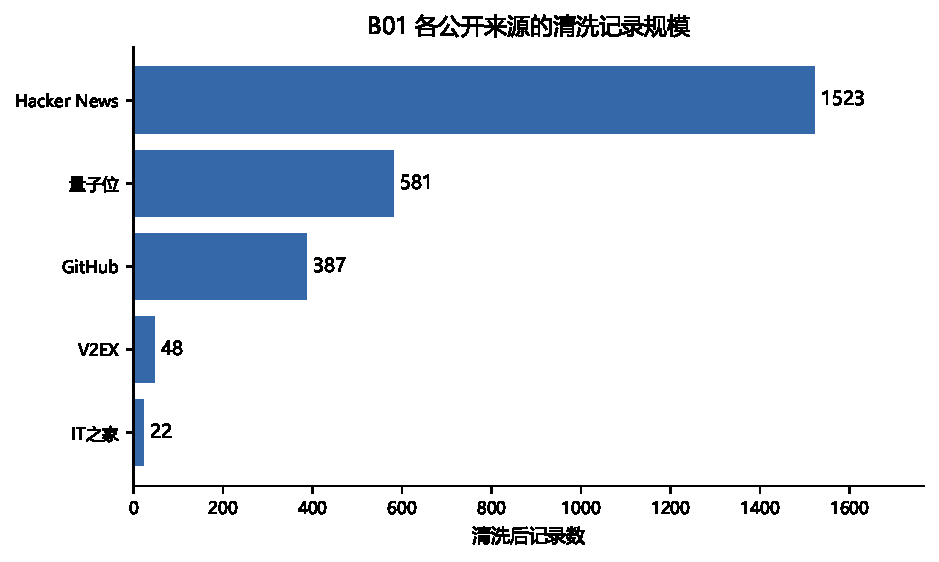
\includegraphics[width=0.86\textwidth]{../figures/fig01_source_counts.pdf}
  \caption{B01 清洗记录的来源规模。Hacker News 占比较高，来源结构存在明显偏斜。}
  \label{fig:sources}
\end{figure}

采集阶段共出现 3,576 次原始字段记录，其中同一来源记录可能因命中多个检索条件而重复。方向筛选排除 742 次字段出现，URL 归并排除 267 条，另有 1 条超出时间窗；得到 2,566 条来源 URL 唯一记录。再按正文证据归并 5 组完全或高度相似内容后，最终保留 2,561 条。来源数量分别为 Hacker News 1,523、量子位 581、GitHub 387、V2EX 48 和 IT之家 22。量子位接口在时间窗内返回的 723 篇记录均已获取；Hacker News、GitHub 搜索和 RSS 入口存在分页或历史覆盖限制，因此本文只把 B01 描述为公开样本批次，不外推平台总体分布。时间覆盖和来源信号的处理也遵循公开指标构造与阶段识别研究中强调的可计算规则\cite{song2020urban}。

\subsection{清洗、去重与质量标记}

清洗过程先对 URL 去除常见追踪参数，再进行 HTML 转文本、Unicode 规范化、空白清理和明显个人信息格式脱敏。重复处理分为同来源 URL 归并、完全相同正文识别和长正文近重复识别；近重复候选使用四字符 TF-IDF 与 shingle Jaccard 联合判断，采用的相似度阈值分别为余弦距离不高于 0.025 和 Jaccard 不低于 0.95\cite{salton1988}。被归并记录仍保留各自来源关系、平台 ID 和热度字段，跨平台指标不相加。该做法延续词项加权用于文本检索与相似性计算的基本思路\cite{salton1988}，但阈值由本批次清洗审计规则固定。

清洗结果中有 670 条内容被标记为不完整，495 条为短文本，907 条没有可用互动指标。图~\ref{fig:quality} 展示这些质量标记；一个记录可能同时命中多个标记。标题、简介和仅标题记录仍保留在数据集中，但在后续机会判别中不允许根据缺失正文外推业务事实。

\begin{figure}[H]
  \centering
  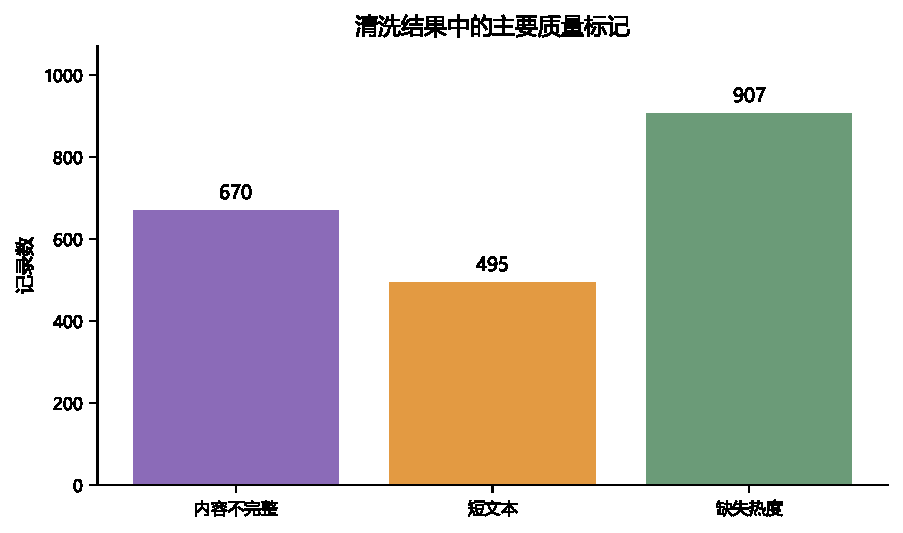
\includegraphics[width=0.82\textwidth]{../figures/fig03_quality_flags.pdf}
  \caption{清洗结果的主要质量标记。一个记录可以同时具有多个标记。}
  \label{fig:quality}
\end{figure}

数据质量审计逐条检查批次号、连续编号、来源链接、时间边界、正文路径、字符数和原始字段关联，JSONL、CSV 与正文快照的记录数均为 2,561。该审计证明处理关系一致，不证明内容相关性或机会标签质量。

采集阶段正文类型包括 \texttt{body} 类型记录 1,796 条、仅标题 396 条、项目简介 274 条、订阅正文 70 条和 README 25 条。\texttt{body} 是采集字段类型，不等同于每条记录都具备完整正文。近重复候选只对足够长的正文进行比较，标题与短文本不因语义相似而自动合并。个人信息清理基于邮箱、电话、IP 和用户名格式识别，无法覆盖所有自然语言线索；因此正文快照保存在本地，公开引用仍以原始来源链接为准。

图~\ref{fig:weekly-sources} 按发布周展示来源记录覆盖，便于区分持续覆盖和单周集中返回。最后一组覆盖至 11 月 7 日，为不完整自然周；Hacker News 的记录量整体较大，资讯与订阅来源的时间分布则受接口历史覆盖范围限制。该图报告的是本批次采集记录，不表示来源平台的实际发帖量。

\begin{figure}[H]
  \centering
  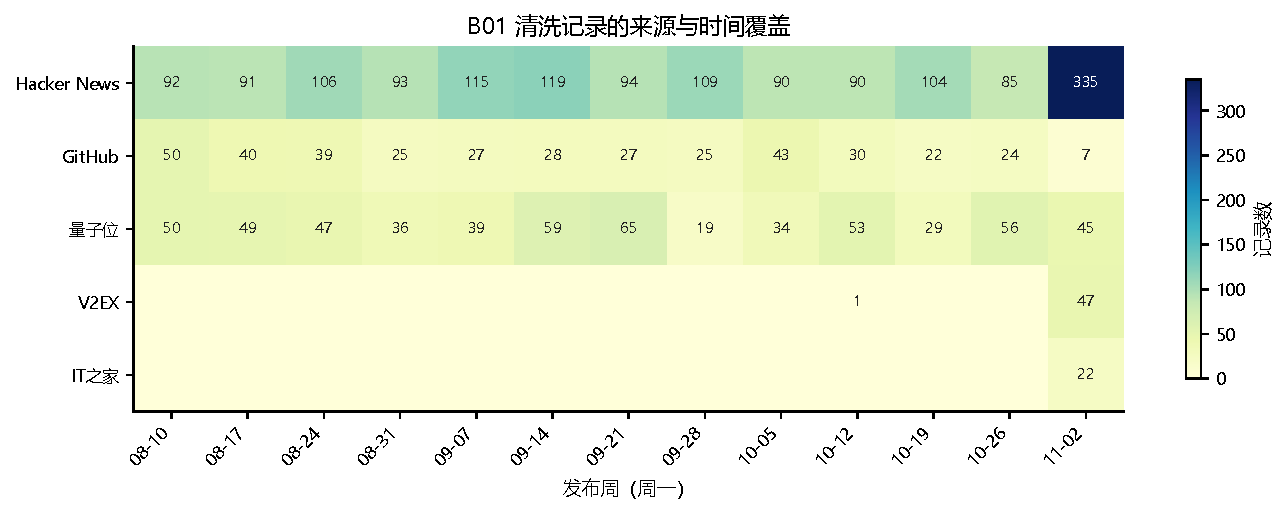
\includegraphics[width=0.98\textwidth]{../figures/fig07_weekly_source_heatmap.pdf}
  \caption{B01 清洗记录的来源与发布周分布。最后一组是截至 2026 年 11 月 7 日的不完整周，计数描述采集样本。}
  \label{fig:weekly-sources}
\end{figure}

不同来源的内容质量标记比例见图~\ref{fig:source-quality}。量子位、V2EX 和 IT 之家记录中热度字段缺失较多；GitHub 则有较高比例的简介型记录。各项比例以来源记录数为分母，缺失热度没有替换为零，质量标记也不会直接改写机会标签。

\begin{figure}[H]
  \centering
  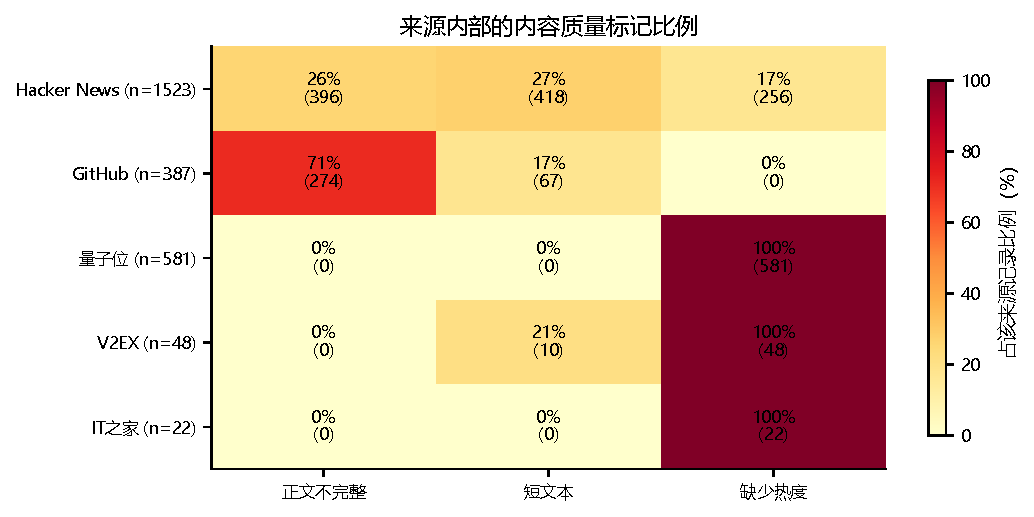
\includegraphics[width=0.88\textwidth]{../figures/fig08_source_quality_heatmap.pdf}
  \caption{来源内部的正文不完整、短文本和缺少热度比例；括号内为对应记录数。一个记录可同时命中多种质量标记。}
  \label{fig:source-quality}
\end{figure}

质量标记不直接改变机会标签；缺失的互动数据也不填为零。后续互动维度仅对实际可用的平台计数进行来源内归一化，以保留不同网站统计单位之间的差异。
